近年、コンピューターの処理速度の向上やデータのデジタル化による扱えるデータの巨
大化などの要因に後押しされ、機械学習の分野の発展は大変著しい。この機械学習の技術を
用いて上記の極端降雨現象の予測に対する新しいアプローチの模索が行われている。

降雨のような時空間データを学習させるための機械学習モデルとしてShi \textit{et al}.[2015]
によってConvLSTM(Convolutional Long-Short Term Memory)が発表された。ConvLSTMは空間的な
特徴を学習させるための機械学習モデルであるCNN(Convolutional Neural Network)と、時間的な
変化を学習させるためのモデルであるLSTM(Long-Short Term Memory)を組み合わせた機械学習モデル
である。具体的な計算式は以下の通りである。

\begin{gather}
  i_{t} = \sigma\left(W_{xi} * X_{t} + W_{hi} * H_{t−1} + W_{ci} \odot \mathcal{C}_{t−1} + b_{i}\right) \\ 
  f_{t} = \sigma\left(W_{xf} * X_{t} + W_{hf} * H_{t−1} + W_{cf} \odot \mathcal{C}_{t−1} + b_{f}\right) \\
  \mathcal{C}_{t} = f_{t} \odot \mathcal{C}_{t−1} + i_{t} \odot \tanh\left(W_{xc} * X_{t} + W_{hc} * \mathcal{H}_{t−1} + b_{c}\right) \\
  o_{t} = \sigma\left(W_{xo} * X_{t} + W_{ho} * \mathcal{H}_{t−1} + W_{co} \odot \mathcal{C}_{t} + b_{o}\right) \\
  \mathcal{H}_{t} = o_{t} \odot \tanh\left(C_{t}\right) 
\end{gather}

さらにConvLSTMの内部構造の概念図以下に示す。

\begin{figure}[H]
\begin{center}
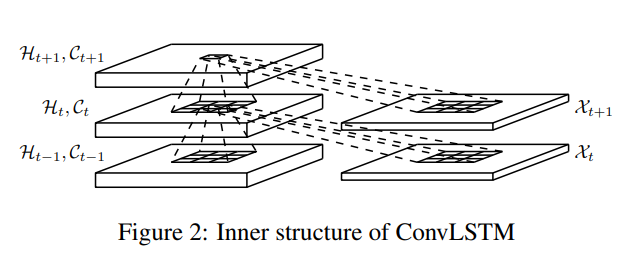
\includegraphics[width=0.8\linewidth]{fig/intro/inner-structure-of-convlstm.png}
\caption{ConvLSTMの内部構造の概念図。Shi \textit{et al}.[2015] Figure2より引用。ConvLSTMの内部構造の概念図。}
\end{center}
\end{figure}

図3の$\mathcal{X}_{t}$・$\mathcal{C}_{t}$・$\mathcal{H}_{t}$はそれぞれ入力・セル状態・
隠れ層の出力を表しており、上記の数式における$X_{t}$・$C_{t}$・$H_{t}$と対応している。
入力は各時刻における入力される空間データを示す。セル状態は過去の状態に関する情報を蓄積
する働きをする。このセル状態が時系列データの効率的な学習を可能としている。計算式(1)
の$i_{t}$は入力ゲートと呼ばれ、入力$X_{t}$と1つ前の時刻の出力$H_{t-1}$に対して畳み込み演算($*$)
が施された結果と1つ前の時刻のセル状態$C_{t-1}$が重み付けされた結果の和をシグモイド関数
を用いて正規化している。さらに計算式(2)の$f_{t}$は忘却ゲートと呼ばれ入力ゲートと同様の計算
が行われれるが、重み$W$が異なっている。計算式(3)の右辺第1項は先ほど求めた忘却ゲートを用いて
過去のセル状態を調整している。右辺第2項は入力ゲートを用いて入力$X_{t}$と1つ前の時刻の出力
$H_{t-1}$の和を調整している。計算式(3)は最終的にこれらを用いてセル状態を更新していること
がわかる。$\odot$はアダマール積を示す。計算式(4)の$o_{t}$は出力ゲートと呼ばれており、
計算式(5)で最終的な出力$H_{t}$を求る際に更新されたセル状態$C_{t}$を調整する働きをしている。

Shi \textit{et al}.[2020]の論文内では降雨のレーダーエコー画像を入力としてConvLSTMモデルを
学習させ一定時間後の降雨の分布と強度の予測を行った。その結果を図2に示す。

\begin{figure}[H]
\begin{center}
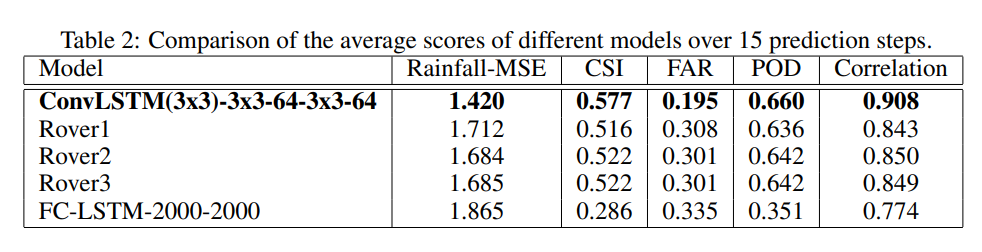
\includegraphics[width=0.8\linewidth]{fig/intro/shi-et-al-convlstm-mse-table.png}
\caption{Shi \textit{et al}.[2015] Table2より引用。ConvLSTM、ROVER、FC-LSTMにおける降雨の予測精度の比較結果。}
\end{center}
\end{figure}

図2の通り、従来手法の一つであるROVER(Real-time Optical flow by Variational methods for Echoes of Radar)
を比較した結果、ConvLSTMモデルは従来手法よりも高い精度で降雨の分布と強度を予測できた。ROVER1・2・3は
モデルの初期化条件を3つのパターンに分けた場合のそれぞれのROVERモデルである。FC-LSTM(fully connected 
LSTM)はLSTMのみを用いて予測を行うモデルである。Rainfall-MSEは予測値と実測値とのMean Squared Error(平均2乗誤差)
、CSI・FAR・PODはそれぞれCritial Success Index・False Alarm Ratio・Probability of Detectionをす。0.5mm/h
以上の降雨が観測OR予測された場合に1、それ以外の場合を0としてそれぞれCSI・FAR・PODを計算した。

この論文が発表されて以来、ConvLSTMを用いた降雨予測の研究が盛んに行われた。Su \textit{et al}.[2020]
の研究ではConvLSTMに降雨のレーダーエコー画像データだけでなく東西・南北風成分を同時に学習させることで
予測のより困難な局所的な対流が原因の降雨の強度や分布の変化を予測できる可能性が示された。本論文の
学習プロセスの概要図を図4に示す。

\begin{figure}[H]
\begin{center}
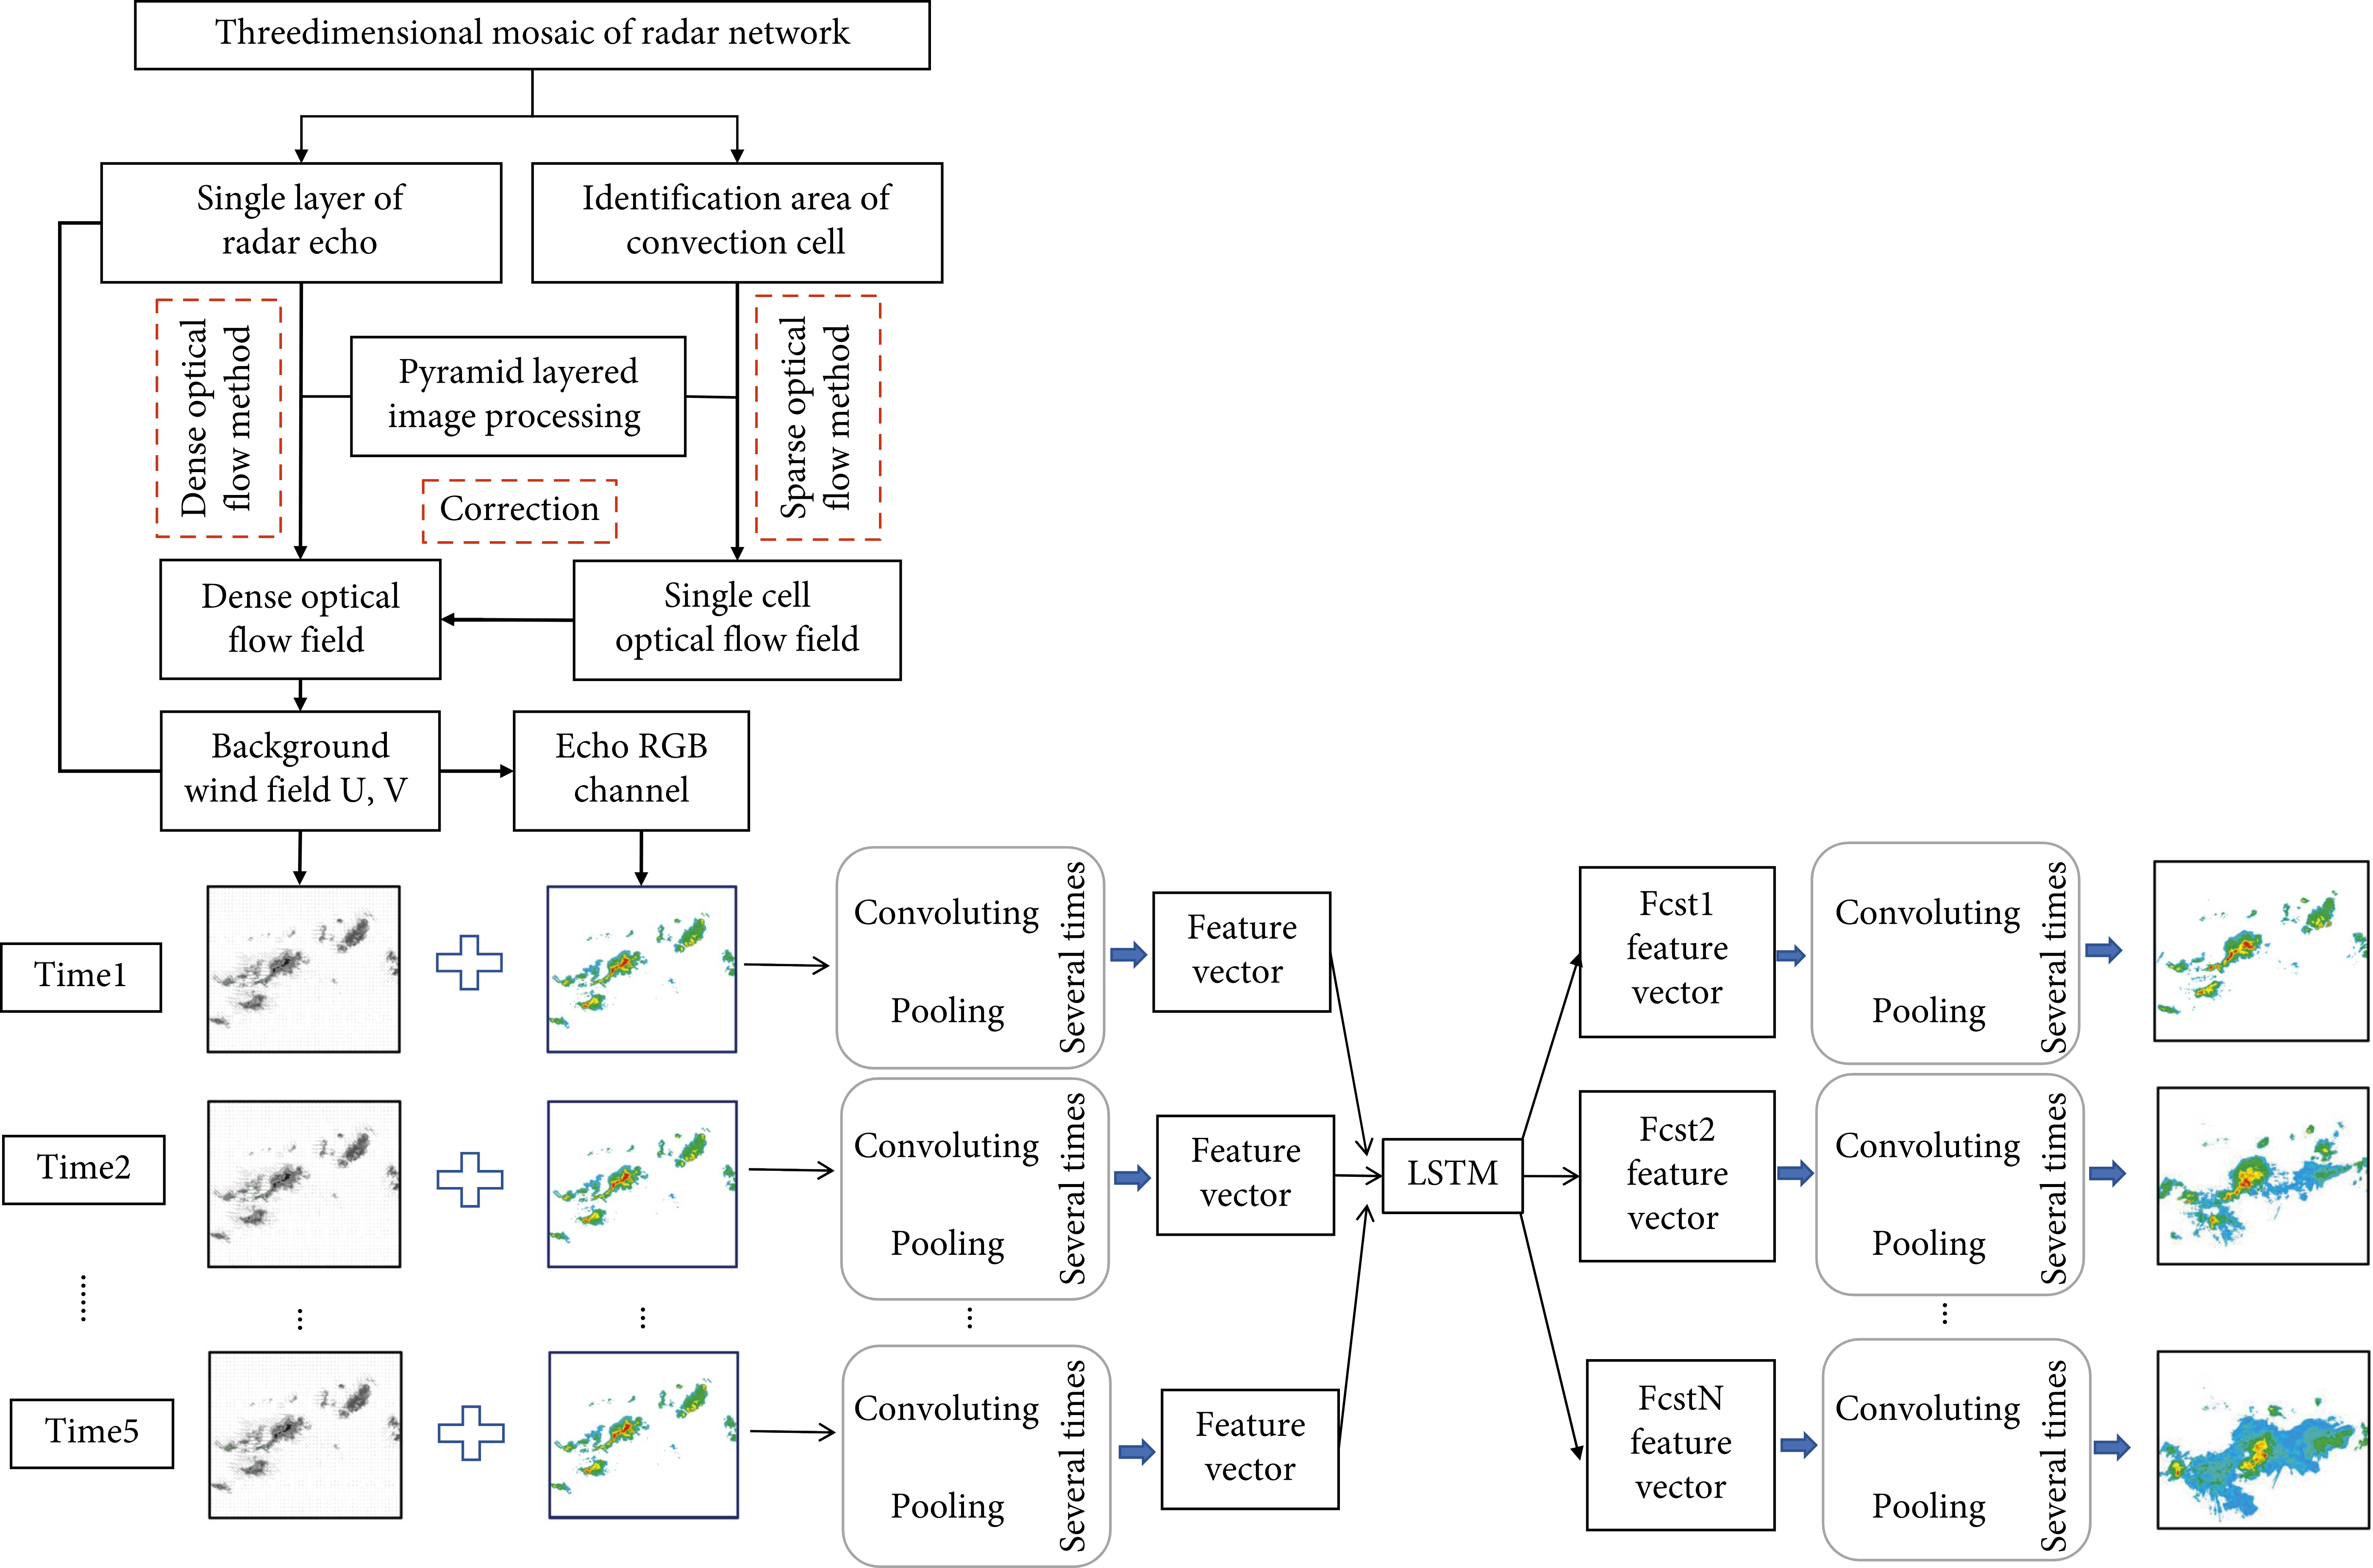
\includegraphics[width=0.8\linewidth]{fig/intro/su-et-al-flowchart.png}
\caption{Su \textit{et al}.[2020] Figure2より引用。降雨と東西・南北風データをConvLSTMに学習させるプロセスの概念図。}
\end{center}
\end{figure}

以下の図5はSu \textit{et al}.[2020]の予測結果の1つである。

\begin{figure}[H]
	\begin{tabular}{cc}
		\begin{minipage}[t]{1.0\hsize}
		\begin{center}
		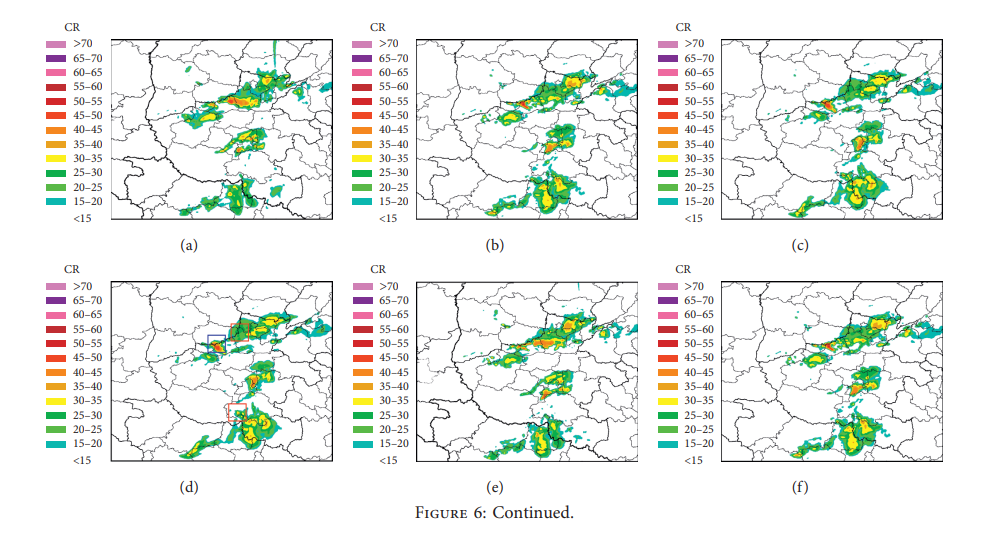
\includegraphics[width=1.0\linewidth,clip]{fig/intro/su-et-al-fig6-1.png}
		\label{a}
		\end{center}
		\end{minipage}\\
		
		\begin{minipage}[t]{1.0\hsize}	
		\begin{center}
		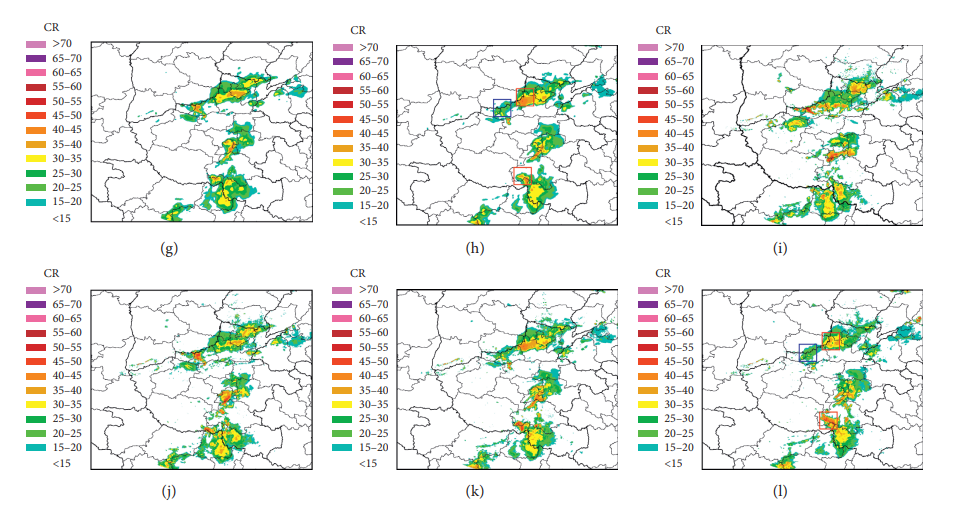
\includegraphics[width=1.0\linewidth,clip]{fig/intro/su-et-al-fig6-2.png}
		\label{b}
		\end{center}
		\end{minipage}
	\end{tabular}
	\caption{Su \textit{et al}.[2020] Figure6より引用。従来手法であるオプティカルフローでの30分・60分・90分・120分後の予測がそれぞれ(a)・(b)・(c)・(d)。ConvLSTMでの30分・60分・90分・120分後の予測がそれぞれ(e)・(f)・(g)・(h)。降雨の30分・60分・90分・120分後の実測画像がそれぞれ(i)・(j)・(k)・(l)。}
\end{figure}

図5の従来手法とConvLSTM予測結果(d), (h)と降雨の実測画像(l)には赤枠と青枠でそれぞれConvLSTMで予測でき、
従来手法で予測できなかった部分とその逆の部分が示されている。このケースのみならず多くの場合において
雨だけでなく風と共に学習させたConvLSTMの方が降雨が強い部分をより多く予測できた結果となった。降雨と
それに関連する気象パラメータを一緒に学習させることで、従来手法では予測が難しかった降雨が予測できる
可能性が示された。

さらに、ConvLSTMの発表をベースにして様々な時空間データを学習させるための機械学習モデルが提案された。
PredRNN (Wang \textit{et al}.[2017b])は水平方向だけでなく鉛直方向成分を持つ時空間データを扱うために
新しいセル状態を導入した。これによって空間のダイナミクスに関する情報をより効率的に学習可能となった。
さらにPredRNN++ (Wang \textit{et al}.[2018b])では

% TODO: honyaku . PredRNN++ (Wang et al. 2018b) increases the transition depth by re-organizing the memories of PredRNN in a cascade fashion.

% TODO: To enhance the ability of PredRNN on modeling high-order dynamics, Memory in Memory (MIM) (Wang et al. 2019) introduces more
% memory cells to process non-stationary and stationary information, which achieves the current SOTA performance in
% spatiotemporal prediction while result in a multiplication of
% computation and memory usage.

そしてSelf-Attention ConvLSTM (Lin \textit{et al}.[2020])が発表され、ConvLSTMや他の派生モデルよりも
高いベンチマークスコアを記録した。このモデルではSelf-Attention機構を導入したことでConvolution処理
では扱えなかったデータ全域に渡る特徴を捉えることができるようになった。さらに過去のSelf-Attention機構
の状態を新しく追加したメモリーモジュールで保管・更新することで時系列に適したモデルとして拡張した。

% TODO: show result and charactaristic of ConvLSTM module.

